\documentclass[10pt]{beamer}
\title[$E_r$-Generating Mechanisms in L-H Transitions]{Comparing Radial Electric Field-Generating Mechanisms in L--H Transitions}
\author[K.A. Blondino]{
\includegraphics[height=1.5cm]{../Graphics/tue_fusion_logo.png} \\ Kevin A. Blondino \\
	Supervisor: dr. H.J. de Blank, TU/e \& DIFFER}
\institute[TU/e]{Eindhoven University of Technology \\
	\medskip
	\textit{k.blondino@student.tue.nl}}
\date{\today}

%{{{ Presentation Style and Color
\mode<presentation>
{
%\usetheme{default}
%\usetheme{AnnArbor}
%\usetheme{Antibes}
%\usetheme{Bergen}
%\usetheme{Berkeley}
\usetheme{Berlin}
%\usetheme{Boadilla}
%\usetheme{CambridgeUS}
%\usetheme{Copenhagen}
%\usetheme{Darmstadt}
%\usetheme{Dresden}
%\usetheme{Frankfurt}
%\usetheme{Goettingen}
%\usetheme{Hannover}
%\usetheme{Ilmenau}
%\usetheme{JuanLesPins}
%\usetheme{Luebeck}
%\usetheme{Madrid}
%\usetheme{Malmoe}
%\usetheme{Marburg}
%\usetheme{Montpellier}
%\usetheme{PaloAlto}
%\usetheme{Pittsburgh}
%\usetheme{Rochester}
%\usetheme{Singapore}
%\usetheme{Szeged}
%\usetheme{Warsaw}

%\usecolortheme{albatross}
\usecolortheme{beaver}
%\usecolortheme{beetle}
%\usecolortheme{crane}
%\usecolortheme{dolphin}
%\usecolortheme{dove}
%\usecolortheme{fly}
%\usecolortheme{lily}
%\usecolortheme{orchid}
%\usecolortheme{rose}
%\usecolortheme{seagull}
%\usecolortheme{seahorse}
%\usecolortheme{whale}
%\usecolortheme{wolverine}

%\setbeamertemplate{caption}[numbered]
\setbeamertemplate{bibliography item}{\insertbiblabel}
%\setbeamertemplate{footline} % To remove the footer line in all slides uncomment this line
%\setbeamertemplate{footline}[page number] % To replace the footer line in all slides with a simple slide count uncomment this line

%\setbeamertemplate{navigation symbols}{} % To remove the navigation symbols from the bottom of all slides uncomment this line
}
%}}}

%{{{ Packages
\usepackage{amsmath,graphicx,booktabs,moresize,textpos}
\usepackage[utf8]{inputenc}
\usepackage{caption}
\captionsetup{labelfont=bf}
\usepackage[UKenglish]{isodate}
\cleanlookdateon
%}}}

% SageTeX!
\usepackage{sagetex}

%{{{ Setup References
\usepackage[backend=bibtex, style=authoryear]{biblatex}
\addbibresource{../References/References.bib}
\renewcommand*{\nameyeardelim}{\addcomma\addspace}
%}}}

%{{{ Two Figures Side-by-Side, separate captions
%\newsavebox\IBoxA \newsavebox\IBoxB \newlength\IHeight
\newcommand\TwoFig[6]{% Image1 Caption1 Label1 Im2 Cap2 Lab2
%	\sbox\IBoxA{#1}
%	\sbox\IBoxB{#4}%
%	\ifdim\ht\IBoxA>\ht\IBoxB
%		\setlength\IHeight{\ht\IBoxB}%
%	\else\setlength\IHeight{\ht\IBoxA}\fi
	\begin{figure}[hbt]
		\minipage[t]{0.48\textwidth}\centering
			{#1}
			\caption{#2}\label{#3}
		\endminipage\hfill\vrule\hfill
		\minipage[t]{0.48\textwidth}\centering
			{#4}
			\caption{#5}\label{#6}
		\endminipage
	\end{figure}%
}
%}}}

%{{{ Two Figures Side-by-Side, with 1 caption
\newcommand\TwoFigOneCap[4]{% Image1 Im2 Caption Label
%	\sbox\IBoxA{#1}
%	\sbox\IBoxB{#2}%
%	\ifdim\ht\IBoxA>\ht\IBoxB
%		\setlength\IHeight{\ht\IBoxB}%
%	\else\setlength\IHeight{\ht\IBoxA}\fi
	\begin{figure}[hbt]
		\minipage[t]{0.48\textwidth}\centering
			{#1}
		\endminipage\hfill
		\minipage[t]{0.48\textwidth}\centering
			{#2}
		\endminipage
		\caption{#3}\label{#4}
	\end{figure}%
}
%}}}

\begin{document}
% Title page
\begin{frame}
\titlepage
\end{frame}

\addtobeamertemplate{frametitle}{}
{
\begin{textblock*}{100mm}(0.85\textwidth,-1cm)
	
\includegraphics[height=1cm,width=2cm]{../Graphics/tue_fusion_logo.png}
\end{textblock*}
}

%--------------------------------------

\begin{frame} % Table of Contents
\tableofcontents
\end{frame}

%--------------------------------------

\section{Bifurcation Theory}
\begin{sagesilent}
	reset()
	var('x,t,a,b')
		# ----------------- Co-dimension 1 ------------------------
	a_min, a_max = -1.5, 0.5
	x_min, x_max = -1.25, 1.25

	# Co-dimension 1 equation
	f1 = diff(x,t) == a + x^2

	co_1 = plot_vector_field((0, f1 / sqrt(a^2 + x^2)), (a, a_min, a_max), (x, x_min, x_max), color='blue', axes=True, frame=True)


	co_1_root = solve(a + x^2 == 0, x)
	co_1_lower = implicit_plot(co_1_root[0], (a,a_min,a_max), (x,x_min,x_max), linewidth=2.5, axes_labels=['$a$','$x$'], color='red', plot_points=2000, gridlines=False, fontsize=20, title="Co-dimension 1 Fold")
	co_1_upper = implicit_plot(co_1_root[1], (a,a_min,a_max), (x,x_min,x_max), linewidth=2.5, color='green', plot_points=2000, figsize=10, typeset='type1')

	# Zero point
	co_1_zero = point((0,0), size=30, color='black')

	co_1_total = co_1_lower + co_1_upper + co_1 + co_1_zero

	# ----------------- Co-dimension 2 ------------------------
	a_min, a_max = -1.2, 1.2
	x_min, x_max = -1.5, 1.5
	var('b')

	# Co-dimension 2 equation
	f2 = diff(x,t) == -(a + b*x - x^3).subs(b=1.1)

	co_2 = plot_vector_field((0, f2), (a, a_min, a_max), (x, x_min, x_max), color='blue', axes=True, frame=True)

	# Points
	turning_point_a = 1/3*sqrt(3)
	turning_point_x = solve(f2.subs(a=turning_point_a), x)[0].right().real()

	co_2_low = implicit_plot(f2.right() == 0, (a, a_min, a_max), (x, x_min, -turning_point_a), linewidth=2.5, color='green', axes_labels=['$a$','$x$'], axes=True, fontsize=20, title="Co-dimension 2 Fold")
	co_2_mid = implicit_plot(f2.right() == 0, (a, a_min, a_max), (x, -turning_point_a, turning_point_a), linewidth=2.5, color='red', axes=True)
	co_2_high = implicit_plot(f2.right() == 0, (a, a_min, a_max), (x, turning_point_a, x_max), linewidth=2.5, color='green', axes=True, figsize=10, typeset='type1')

	arrow_up = arrow((0.48, -0.55), (0.48, 1.2), width=3, color='black')
	arrow_down = arrow((-0.48, 0.55), (-0.48, -1.2), width=3, color='black')

	#co_2_zero1 = point((turning_point_a, turning_point_x), size=40, color='black')
	#co_2_zero2 = point((-turning_point_a, -turning_point_x), size=40, color='black')

	co_2_total = co_2 + co_2_low + co_2_mid + co_2_high + arrow_up + arrow_down
\end{sagesilent}
\begin{frame} % Bifurcation Theory, Co-dimension 1
\frametitle{Bifurcation Theory}
\begin{figure}[h]
\begin{minipage}{0.49\linewidth}
	\centering
	\sageplot[width=\linewidth]{co_1_total}
\end{minipage}
\begin{minipage}{0.49\linewidth}
	Bifurcation -- A topological or qualitative change in a system when a smooth change of parameter is made. \vspace*{5mm}
	\caption{Plot of steady-state of $\dot{x} \,=\, a \,+\, x^2$; red is unstable, green is stable}
\end{minipage}
\end{figure}

\end{frame}

%--------------------------------------

\begin{frame} % Co-dimension 2, Hysteresis
\frametitle{Bifurcation Theory}
\begin{figure}[h]
\begin{minipage}{0.49\linewidth}
	\centering
	\sageplot[width=\linewidth]{co_2_total}
\end{minipage}
\begin{minipage}{0.49\linewidth}
	Hysteresis -- the dependence of a state on the history of the system. \vspace*{5mm}
	\caption{Plot of steady-state of $\dot{x} \,=\, -(a \,+\, bx \,-\, x^3)$; red is unstable, green is stable}
\end{minipage}
\end{figure}
\end{frame}

%--------------------------------------

\begin{sagesilent} # SHOW ZEROS!
	reset()

	var('x, a, b, x_dot,t')
	x_min, x_max = -2.0, 2.0

	"""
		ROOT FINDING function, for all of the roots.
		Returns a sorted list of UNIQUE roots. This does NOT work when there
		is multiplicity in the roots. Use `w.roots()` to symbolically check
		for multiplicity.
	"""
	def find_root_recursive(func, lower_bound, upper_bound, tol=1.0e-12):
	    L = []
	    try:
	    	x0 = find_root(func, lower_bound, upper_bound)
	    	L.append(x0)
	    	L += find_root_recursive(func, lower_bound, x0-tol, tol)
	    	L += find_root_recursive(func, x0+tol, upper_bound, tol)
	    except:
	    	pass
	    return L

	# ----------------- \dot{x} vs x plots --------------------
	x_dot = -(a + b*x - x^3)

	a_list = [-2.0, 0.0, 2.0]

	plot_list = []
	point_list = []

	the_title = "$\dot{x} = -(a + bx - x^3)$"
	ax_labels = ["$x$", r"$\dot{x}$"]
	the_font_size = 54

	b_selection = -0.8

	## The one with only one zero
	for i in range(len(a_list)):
	    this_loops_color = rainbow(len(a_list)+2)[i+2]

	    the_label = "$a = " + str(a_list[i].n(prec=10)) + "$"

	    plot_list.append(plot(x_dot.subs(a=a_list[i], b=b_selection),\
	    		(x, x_min, x_max), color=this_loops_color, gridlines='major',\
	    		title=the_title, thickness=4.0, frame=True, axes=False,\
	    		legend_label=the_label, axes_labels=ax_labels, figsize=16,\
	    		fontsize=the_font_size, typeset='type1'))

	    # Create list of points of zeros
	    particular_roots = find_root_recursive(x_dot.subs(a=a_list[i], b=b_selection), x_min, x_max)

	    for j in particular_roots:
	    	point_list.append(ellipse((j,0), 0.04, 0.22, color=this_loops_color,\
	    			thickness=4.0, aspect_ratio='automatic'))

	# Create the parameter box for b
	b_parameter_box1 = text('$b = ' + str(b_selection.n(prec=8)) + '$',\
			(x_max-0.1, -10.0), bounding_box={'boxstyle':'round', 'fc':'w'},\
			fontsize=the_font_size, color='black', horizontal_alignment='right')

	combined_plots1 = sum(plot_list) + sum(point_list) + b_parameter_box1
	combined_plots1.set_legend_options(font_size=the_font_size)


	## The one with 2 or 3 zeros
	# Reset the plot and point lists
	plot_list = []
	point_list = []

	b_selection = 1.1
	ax_labels=["$x$", ""]

	for i in range(len(a_list)):
	    this_loops_color = rainbow(len(a_list)+2)[i+2]

	    the_label = "$a = " + str(a_list[i].n(prec=10)) + "$"

	    plot_list.append(plot(x_dot.subs(a=a_list[i], b=b_selection),\
	    		(x, x_min, x_max), color=this_loops_color, gridlines='major',\
	    		thickness=4.0, frame=True, axes=False,\
	    		title=the_title, axes_labels=ax_labels, figsize=16,\
	    		fontsize=the_font_size, typeset='type1'))

	    # Create list of points of zeros
	    particular_roots = find_root_recursive(x_dot.subs(a=a_list[i], b=b_selection), x_min, x_max)
	#	particular_roots = [find_root(x_dot.subs(a=a_list[i], b=b_selection), x_min, x_max)]
	    for j in particular_roots:
	    	point_list.append(ellipse((j,0), 0.03, 0.2, color=this_loops_color,\
	    			thickness=4.0, aspect_ratio='automatic'))


	# Create the parameter box for b
	b_parameter_box3 = text('$b = ' + str(b_selection.n(prec=10)) + '$',\
			(x_max-0.1, -6.8), bounding_box={'boxstyle':'round', 'fc':'w'},\
			fontsize=the_font_size, color='black', horizontal_alignment='right')


	# Tangent root function
	tangent_root_fun = x_dot.subs(a=sqrt(4*b_selection^3/27), b=b_selection)

	# Equation with exactly 2 ROOTS
	plot_list.append(plot(tangent_root_fun, (x, x_min, x_max), color='black',\
			legend_label=r'$a = \sqrt{\frac{4\,b^3}{27}}$', thickness=4.0))

	## Find lower, tangent root
	point_list.append(ellipse((find_root(tangent_root_fun, x_min, 0),0), 0.03,\
			0.2, color='black', thickness=4.0, aspect_ratio='automatic'))

	# Find upper, non-tangent root, and make point
	point_list.append(ellipse((find_root_recursive(tangent_root_fun, 0, x_max)[0],\
			0), 0.03, 0.2, color='black', thickness=4.0, aspect_ratio='automatic'))

	combined_plots3 = sum(plot_list) + sum(point_list) + b_parameter_box3
	combined_plots3.set_legend_options(font_size=the_font_size, loc='upper left')

\end{sagesilent}
\begin{frame} % Bifurcation Theory zeros
\frametitle{Bifurcation Theory}
\TwoFigOneCap{\sageplot[width=1.0\textwidth]{combined_plots1}}
	{\sageplot[width=1.0\textwidth]{combined_plots3}}
	{Phase plots of co-dimension 2 bifurcation with different values of $a$ within each plot. %
	There is a variance in the number of zeros based on the values of $a$ in the right plot, while there is strictly one zero for all values of $a$ in the left plot.}
	{fig:stationaries_b}
\end{frame}

%--------------------------------------

\begin{sagesilent}
	reset()

	var('x,t,a,b')
	# ----------------- Co-dimension 2 ------------------------
	a_min, a_max = -1.1, 1.1
	x_min, x_max = -1.4, 1.4
	var('b')

	# Co-dimension 2 equation
	f2 = diff(x,t) == -(a + b*x - x^3)

	the_axes_labels = ['$a$','$x$']
	the_figsize = 10
	the_title = "Co-dimension 2 Fold"
	the_linewidth = 2.0
	the_fontsize = 20

	b_values = [-0.5, 0.0, 1.0]
	b_plots = []
	the_label = []
	the_colors = rainbow(len(b_values))

	for i in range(len(b_values)):

	    b_plots.append(implicit_plot(f2.right().real().subs(b=b_values[i]) == 0,\
	    		(a, a_min, a_max), (x, x_min, x_max), linewidth=the_linewidth,\
	    		color=the_colors[i], axes_labels=the_axes_labels,\
	    		axes=True, gridlines=True, figsize=10, aspect_ratio=0.8,\
	    		fontsize=the_fontsize, title=the_title, typeset='type1'))

	boxes = [text('$b = -0.5$', (0.9, 0.7),\
			bounding_box={'boxstyle':'round', 'fc':'w'},\
			fontsize=the_fontsize-4, color='black')]
	boxes.append(text('$b = 0.0$', (0.95, 1.0),\
			bounding_box={'boxstyle':'round', 'fc':'w'},\
			fontsize=the_fontsize-4, color='black'))
	boxes.append(text('$b = 1.0$',(0.25, 1.2),\
			bounding_box={'boxstyle':'round', 'fc':'w'},\
			fontsize=the_fontsize-4, color='black'))
	boxes.append(text('$a - bx + x^3 = 0$', (0.6, -1.3),\
			bounding_box={'boxstyle':'round', 'fc':'w'},\
			fontsize=the_fontsize, color='black'))

	combined_plots = sum(b_plots) + sum(boxes)
\end{sagesilent}
\begin{frame} % Surface of varying b
\frametitle{Bifurcation Theory}

\TwoFigOneCap{\sageplot[width=\textwidth]{combined_plots}}
	{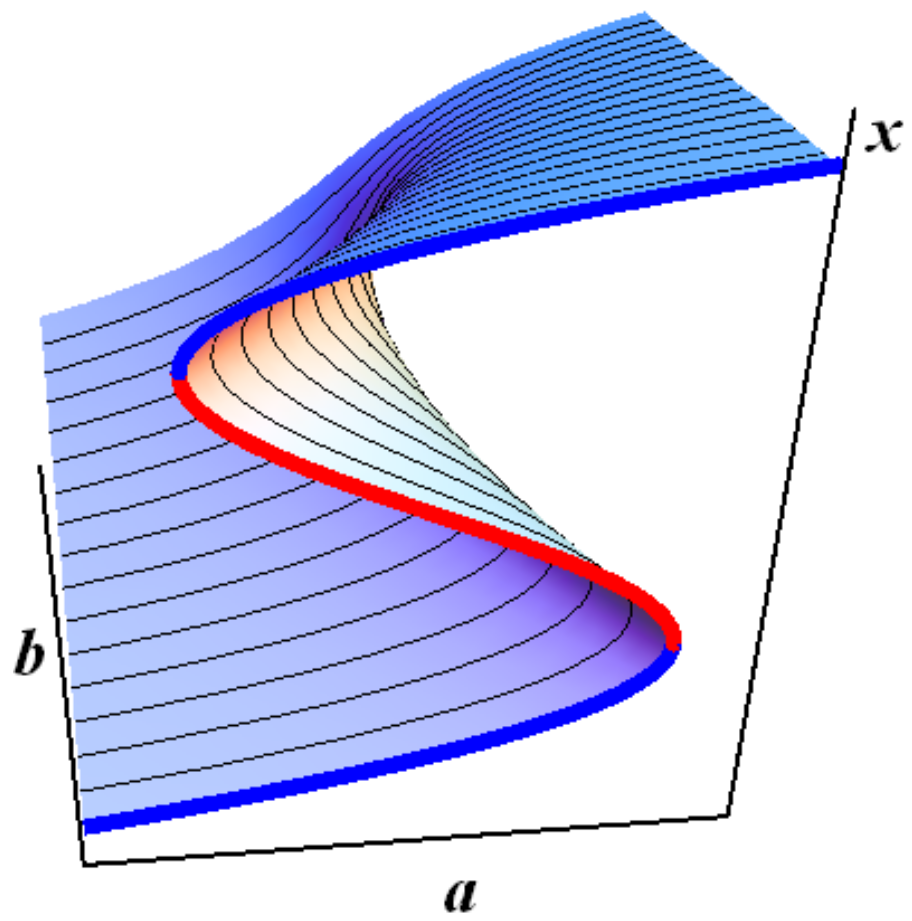
\includegraphics[width=0.95\textwidth]{../Graphics/Bif_Graphs/Bif_3D.png}}
	{These plots show the mentioned co-dimension 2 cusp bifurcation, composed of two co-dimension 1 fold bifurcations.
	The plot on the right is the surface plot of this same model \parencite{weymiens_bifurcation_2014}.}
	{fig:Bif_hysteresis}

\end{frame}

%--------------------------------------

\begin{frame} % Co-dimension 3
\frametitle{Bifurcation Theory}

\begin{figure}[tb] % Co-dimension 3 bifurcation cross-section
\begin{minipage}{0.59\linewidth}
	\centering
	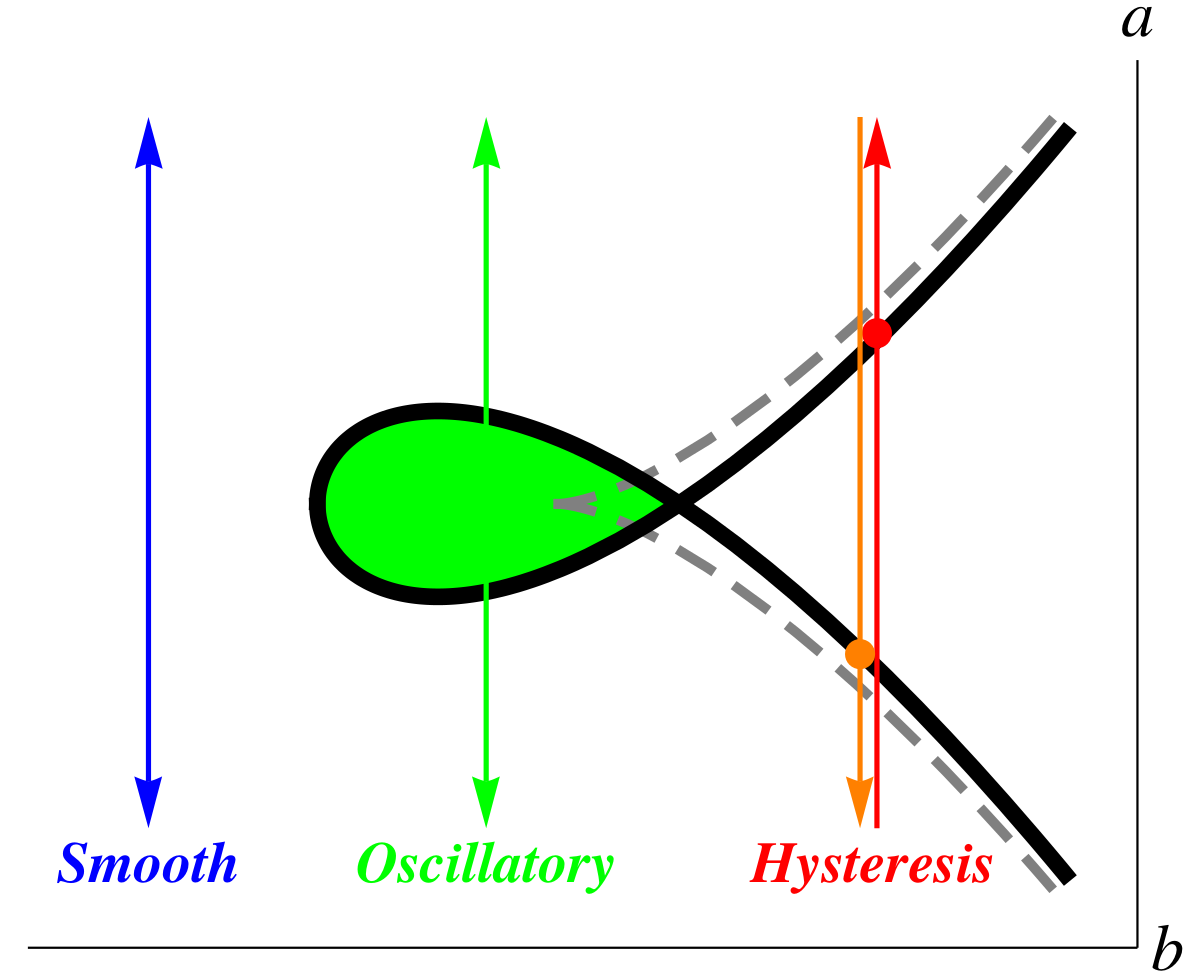
\includegraphics[width=\textwidth]{../Graphics/Bif_Graphs/3_transitions_single_simple.png}
\end{minipage}
\hfill
\begin{minipage}{0.39\linewidth}
	\caption{FitzHugh-Nagumo model, a co-dimension 3 bifurcation with the black line indicating the fold bifurcation.
	It accurately describes the L--H transition in tokamak plasmas, with the $b$ parameter dictating the type of transition \parencite{weymiens_bifurcation_2014}.}
	\label{fig:co-3}
\end{minipage}
\end{figure}

\end{frame}

%--------------------------------------

\section{H--mode}
\begin{frame} % First H--mode slide
\frametitle{H--mode}

\begin{itemize}
	\item The L--H transition is a bifurcation of anomalous transport at the edge. High auxiliary power develops strong sheared $\mathbf{E}\times\mathbf{B}$-drift plasma flow \parencite{terry_suppression_2000}.
	\item Experiments at TEXTOR showed that a biased probe produced H--mode \parencite{weynants_confinement_1992}.
\end{itemize}

\begin{figure}[tb] % L--H-modes compare
\begin{minipage}{0.59\linewidth}
	\centering
	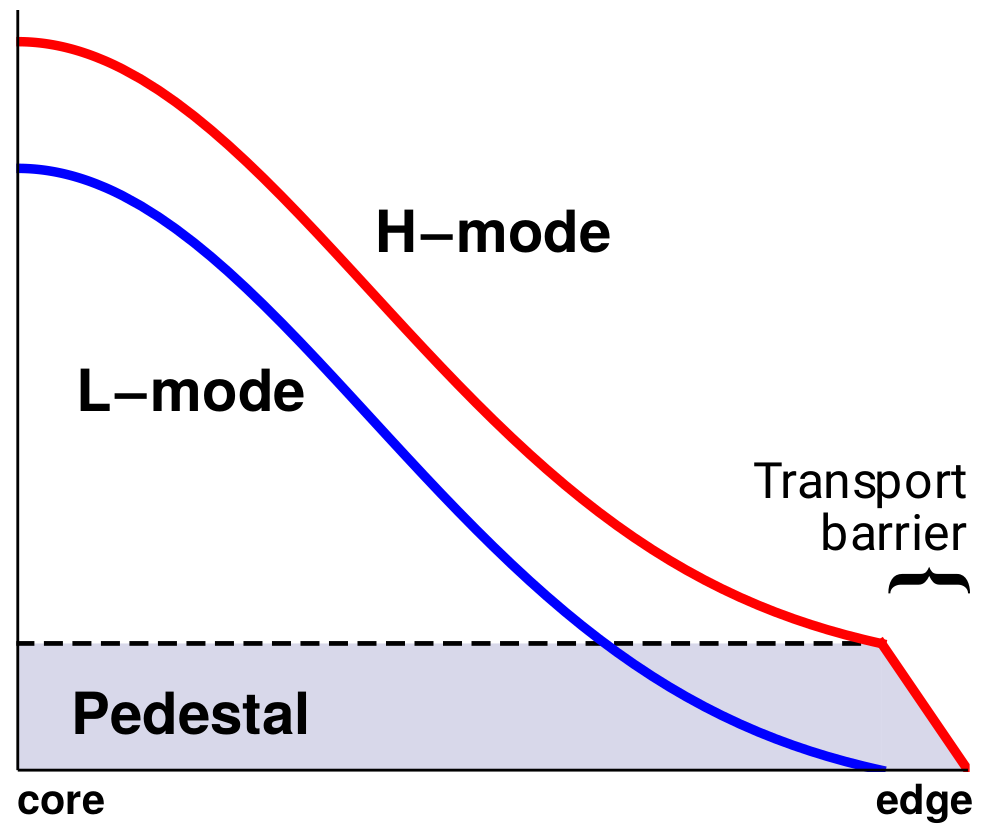
\includegraphics[width=0.75\textwidth]{../Graphics/L-mode_H-mode_compare.png}
\end{minipage}
\hfill
\begin{minipage}{0.39\linewidth}
	\caption{A comparison of the radial pressure profiles of L--mode and H--mode \parencite{weymiens_bifurcation_2014}.}
	\label{fig:L-mode_H-mode_compare}
\end{minipage}
\end{figure}

\end{frame}

%--------------------------------------

\begin{frame} % Radial Electric Field
\frametitle{Radial Electric Field}
\begin{equation} % Lorentz Force Balance
	E_r \,=\, -\frac{1}{n_j e_j} \frac{\text{d} p_j}{\text{d} r} + V_{\theta j} B_\phi - V_{\phi j} B_\theta
	\label{eq:E_r}
\end{equation}
\begin{itemize}
	\item $V_{\theta j}$ and $V_{\phi j}$ are unreasonably-difficult to measure.
	\item Instead, look at nonambipolar particle fluxes that can be calculated by the electric field, density, temperature, and their gradients.
\end{itemize}
\begin{align} % Ambipolarity constraint
	\epsilon_0 \frac{\partial E_r}{\partial t} \,=\, -\sum J_r \,=\,
		\sum_\text{k} q_j\Gamma_j^\text{k} \label{eq:ambipolarity_constraint}
\end{align}
\begin{itemize}
	\item It is useful to normalize the field to the gyroradius and temperature.
\end{itemize}
\begin{align} % Z definition
	Z \,\equiv\, \frac{\rho_{\theta i} \, e \, E_r}{T_i}~, ~~~~
		\rho_{\theta i} \,\equiv\, \frac{m_i \, v_{T_i}}{e \, B_\theta}
		\label{eq:Z_and_rho_definitions}
\end{align}
\end{frame}

%--------------------------------------

\section{Dynamical Model}
\begin{frame}
\frametitle{Dynamical Model: Transport Equations}
\begin{itemize}
	\item Conservation of mass
\begin{align} % n continuity
	\frac{\partial n}{\partial t} \,=\, -\frac{\partial \Gamma}{\partial x}~,
		~~~ \Gamma \,=\, -D \, \frac{\partial n}{\partial x}
		\label{eq:n_continuity}
\end{align}
	\item Conservation of energy
\begin{align} % U continuity
	\frac{\partial U}{\partial t} \,=\, \frac{\partial}{\partial t}
		\left(\frac{n\,T}{\gamma - 1}\right) \,=\,
		-\frac{\partial q}{\partial x}~, \label{eq:U_continuity} \\
	q \,=\, -\chi \, n \, \frac{\partial T}{\partial x} \,+\,
	\frac{\Gamma \, T}{\gamma - 1}~,~~~ \chi \,=\, \frac{D}{\zeta (\gamma - 1)}
\end{align}
	\item Compact Equations
\begin{align} % More reduced temperature equation
	\dot{n} \,=\, \frac{\partial}{\partial x} \left[D \, n^\prime\right]~,~~~
	\dot{T} \,=\, \frac{\partial}{\partial x}\left[\frac{D}{\zeta} \,
		T^\prime\right] \,+\, \left(1 + \frac{1}{\zeta}\right) n^\prime \,
		T^\prime \label{eq:transport_eqs_compact}
\end{align}
\end{itemize}
\end{frame}

%--------------------------------------

\begin{frame}
\frametitle{Dynamical Model: Nonambipolar Fluxes}
A total of 6 fluxes were investigated:
\begin{align}
	\text{Polarization Current:}~~ J^\text{pol} \,&=\, \frac{e \, n \, \rho_{\theta i}}{2} \,
		\frac{\partial Z}{\partial t} \label{eq:polarization_current_normalized} \\
	\text{Ion Shear Viscosity:}~~ J^{\pi\perp} \,&=\, -\frac{e \, \rho_{\theta i}}{2} \,
		\frac{\partial}{\partial x} \left[\mu \, n \, \frac{\partial Z}
		{\partial x}\right] \label{eq:shear_current_normalized} \\
	\text{Ion Bulk Viscosity:}~~ \Gamma_i^{\pi\parallel} \,=\, \,n_e\,&D_{\pi\parallel}
		\left(\frac{n^\prime}{n} + \frac{Z}{\rho_{\theta i}}\right) \,
		\text{Im}\left[X\left(Z \,+\, i\,\frac{\nu_{ii}}{\omega_t}\right)\right]
		\label{eq:stringer_Gamma_bulk} \\
	&D_{\pi\parallel} \,=\, \frac{\epsilon^2\,\rho_{\theta i}\,T}
		{(x - a_m)\sqrt{\pi}\,B} \label{eq:stringer_D_bulk} \\
	\text{Anomalous Electron Loss:}~~ \Gamma_e^\text{an} \\
	\text{Charge Exchange Friction:}~~ \Gamma_i^\text{cx} \\
	\text{Ion Orbit Loss:}~~ \Gamma_i^\text{ol}
\end{align}
\end{frame}

%--------------------------------------

\section{Results}
\begin{frame}
	This is a test!
\end{frame}

%--------------------------------------

\begin{frame}
	This is a test!
\end{frame}

%--------------------------------------

\begin{frame}
	This is a test!
\end{frame}

%--------------------------------------

%\section{References}
\begin{frame}
\frametitle{References}
\renewcommand*{\bibfont}{\tiny}
%\nocite{*}
\printbibliography
\end{frame}
%}}}

%--------------------------------------
\end{document}

